\documentclass[preprint,12pt,numbers]{elsarticle}
\usepackage{amsmath,amssymb,amsthm,booktabs,graphicx,microtype,float,etoolbox}
\AtBeginEnvironment{thebibliography}{\small}
\setlength{\emergencystretch}{2em}
\usepackage{multirow}
\usepackage{tikz}
\usetikzlibrary{positioning,arrows.meta,calc,fit}
\definecolor{paletteBlue}{HTML}{74A9C5}
\definecolor{paletteMint}{HTML}{C2E5CF}
\definecolor{paletteYellow}{HTML}{EDDDAB}
\definecolor{paletteCoral}{HTML}{F2B8AE}
\definecolor{paletteRose}{HTML}{DD7389}
\colorlet{paletteBlueEdge}{paletteBlue!80!black}
\colorlet{paletteBlueFill}{paletteBlue!18}
\colorlet{paletteMintEdge}{paletteMint!70!black}
\colorlet{paletteMintFill}{paletteMint!42}
\colorlet{paletteYellowEdge}{paletteYellow!75!black}
\colorlet{paletteYellowFill}{paletteYellow!38}
\colorlet{paletteCoralEdge}{paletteCoral!80!black}
\colorlet{paletteRoseText}{paletteRose!70!black}
\usepackage[hidelinks]{hyperref}
\usepackage{xurl}
\newcommand{\E}{\mathbb{E}}
\newcommand{\Var}{\operatorname{Var}}
\newcommand{\Z}{\mathbb{Z}}
\newtheorem{theorem}{Theorem}
\newtheorem{lemma}{Lemma}
\newtheorem{corollary}{Corollary}
\newtheorem{proposition}{Proposition}
\theoremstyle{definition}
\newtheorem{definition}{Definition}
\journal{Integration, the VLSI Journal}

\begin{document}
\begin{frontmatter}
\title{Carry Conservation in Approximate Accumulators: Quantizer Equivalence and an Entropy Bound}
\author[nyu]{Rei Li\corref{cor1}\fnref{orcid1}}
\ead{reili2isak@gmail.com}
\author[nyu]{Xinyi Li\fnref{orcid2,co_second}}
\ead{lieve7154@gmail.com}
\author[rochester]{Ivy Li\fnref{orcid3,co_second}}
\ead{ivy621550011@gmail.com}
\cortext[cor1]{Corresponding author.}
\fntext[orcid1]{ORCID: 0009-0003-3471-5370.}
\fntext[orcid2]{ORCID: 0009-0002-6985-7005.}
\fntext[orcid3]{ORCID: 0009-0002-9031-4259.}
\fntext[co_second]{Xinyi Li and Ivy Li contributed equally as second authors.}
\affiliation[nyu]{organization={New York University Tandon School of Engineering},
  city={Brooklyn}, postcode={11201}, state={New York}, country={United States of America}}
\affiliation[rochester]{organization={University of Rochester},
  city={Rochester}, state={New York}, country={United States of America}}

\begin{abstract}
An accumulator feeds its previous output into its adder, so single-addition
error need not predict accumulated error.
For lower-part adders, accumulated error equals the sum of carries into
the upper part, weighted by $2^k$, minus operand residues, up to a
bounded low-register term. If the carry ignores the low state, the
design equals exact accumulation of quantized operands on every input
sequence, and its low part can be removed. Otherwise, under uniform
residues, low state buys at most its entropy rate in accuracy; rounding
attains this bound. Across 89 certified designs (with residue properties
proved by exhaustive enumeration or SAT), Nangate45 synthesis,
place and route at two clocks with gate-level power, and an FPGA,
lower-part adders cost a median 9--19\% more area and energy than the
cheapest equally accurate exact accumulator of rounded or truncated
operands. No design is more than 8\% cheaper. In INT8 ResNet-20
inference, accumulating rounded products is cheapest within one
accuracy point of exact accumulation. It saves 40\% routed area on
CIFAR-10 and 33\% in a CIFAR-100 replication with a protocol fixed
before training. New accumulator designs should first be compared
with exact accumulation of rounded operands at similar accuracy.
\end{abstract}

\begin{keyword}
approximate adders \sep accumulators \sep quantization \sep VLSI
\end{keyword}
\end{frontmatter}

\section{Introduction}

Accumulation is the inner loop of multiply--accumulate (MAC) units, finite
impulse response (FIR) filters, and neural network dot products.
An accumulator adds a fresh operand to its previous result, and each output
becomes the next input of the same adder. Many approximate
adders have been proposed to reduce the cost of this
datapath~\cite{xu2016survey,mittal2016survey}. Most are \emph{lower-part}
designs that replace the low $k$-bit circuit with a cheaper one and
pass at most a carry to an exact upper
part~\cite{mahdiani2010loa,zhu2010eta,gupta2013ama,albicocco2012loawa}. Their
quality is reported with single-addition metrics such as mean error distance
or mean squared error under uniform
inputs~\cite{liang2013metrics,mrazek2017evoapprox}.

Single-addition metrics omit feedback through the low register, whose value
after one addition becomes an input to the next.
Earlier studies found error buildup in approximate sequential
circuits and showed that isolated metrics can
mislead~\cite{miao2012dither,kapare2016seq,chandrasekharan2016seq,park2021mac}.
We examine which part of an adder's behavior survives accumulation and
what accuracy its hardware state can support.
Barrois et al.\ found on benchmarks that reducing word length was usually a
cheaper way to trade accuracy than approximate operators~\cite{barrois2017hidden}.
A benchmark comparison leaves open whether an untested cell could reverse
that finding and which existing cells are redundant. For lower-part accumulators, we answer
both questions by proof, stating whether each result holds pathwise or under an input law.

We derive a carry conservation law for lower-part adders in
Lemma~\ref{lem:conservation}. It expresses accumulated error as
$q=2^k$ times the delivered carries minus the operand residues, plus a
bounded difference between the final and initial low-register values.
Low-sum error remains in the register and affects later additions, explaining
why isolated metrics can mislead. From the identity,
we derive pathwise quantizer equivalence, removable logic, exact error
metrics, an optimal state-blind quantizer, and an entropy bound attained
by rounding.
Our contributions are as follows:
\begin{itemize}
\item We show that a state-blind carry makes accumulation pathwise
equivalent, within $q$, to exact accumulation of a
quantized operand (Theorem~\ref{thm:blind}). Its low part can be removed
without changing the upper bits (Corollary~\ref{cor:prune}).
A threshold quantizer is best among these designs for any independent
operand law. The lower-part OR adder~\cite{mahdiani2010loa} reads the state
but is pathwise equivalent to round-half-up.
\item We derive drift (mean error per addition), diffusion (long-run variance
growth per addition), and
finite-length MSE from a $q\times q$
table for any independent residue law (Theorem~\ref{thm:moments}). Under uniform residues, low state
provides at most $h$ bits of accuracy gain, where $h$ is its entropy rate.
Rounding attains this bound at every integer $h$ (Theorem~\ref{thm:bound}),
while a machine-specific bound applies to other laws
(Theorem~\ref{thm:lawbound}).
\item We classify 89 designs whose residue property is proved by exhaustive
enumeration or SAT (Section~\ref{sec:census}) and
prove quantizer-twin equivalence for 1440 extracted netlists
(Section~\ref{sec:blindhw}). We evaluate Nangate45 synthesis, place and
route at two clocks with gate-level power, and an FPGA. Approximate
designs have a median 9--19\% penalty against equally accurate reference
accumulators, defined as exact accumulation of rounded or truncated operands.
\item We evaluate bit-exact INT8 ResNet-20 inference, where accumulating
rounded products is cheapest at the one-point criterion
(Section~\ref{sec:cnn}). A CIFAR-100 replication with a protocol fixed
before training confirms the cost ordering. We also test a long FIR
filter on real images.
\end{itemize}
Section~\ref{sec:related} reviews related work.
Sections~\ref{sec:model} and~\ref{sec:theory} present the model and theory.
Sections~\ref{sec:census}--\ref{sec:cnn} report the design census,
hardware evaluation, and applications. Section~\ref{sec:discussion}
discusses limitations.

\section{Related work}
\label{sec:related}

\paragraph{Lower-part approximate adders and their analysis}
The lower-part OR adder (LOA) computes low bits with OR gates and
forwards the AND of the most significant low bits as a
carry~\cite{mahdiani2010loa}. LOAWA (LOA without the AND gate) omits
that carry~\cite{albicocco2012loawa}. Error-tolerant adder type I
(ETA-I)~\cite{zhu2010eta} saturates the low
bits below the first position where both operands are one.
Approximate mirror adders (AMA), including AMA2 and AMA5, replace
full-adder cells~\cite{gupta2013ama}.
Evolutionary design produced the EvoApproxLib library~\cite{mrazek2017evoapprox}.
New cells continue to receive single-addition
evaluations~\cite{echavarria2017aer,huang2026sfe}. Carry-speculative adders
such as ETA-II~\cite{zhu2009eta} segment the carry chain. Their error
depends on high operand bits, placing them outside the class studied here.
Analytical and probabilistic models characterize one addition or a fixed
adder network~\cite{liang2013metrics,liu2015analytical,mazahir2017probabilistic,li2014errormodel,ayub2017statistical,ayub2021peal,hanif2020pemacx,hanif2023daem,hanif2024dreamx},
and formal methods count the errors of a fixed combinational
circuit~\cite{venkatesan2011macaco,abed2020satmetrics,meng2024vacsem,ramprasath2026mcac}.
These analyses treat combinational circuits, whereas accumulator feedback
through the same adder requires a sequential model.

\paragraph{Approximation in sequential and MAC datapaths}
Miao et al.\ identified error buildup in chained additions and introduced
dithering adders~\cite{miao2012dither}. Kapare et al.\ fitted error
trends of approximate accumulators~\cite{kapare2016seq}.
Chandrasekharan et al.\ computed accumulated worst-case errors by model
checking~\cite{chandrasekharan2016seq}. ASLAN synthesizes approximate
sequential circuits under accumulated-quality
constraints~\cite{ranjan2014aslan}. Park et al.\ interleaved multipliers with
opposite biases~\cite{park2021mac}. Control-variate approximation adds a
correction term per accumulation to cancel the expected error of approximate
multipliers~\cite{zervakis2021cv}. Our calibrated preload plays the same role
for the accumulator's own drift and is computed exactly by
Theorem~\ref{thm:moments}. CANN defers missed carries between MAC segments to
a later cycle~\cite{cann_curable}. Dharmaraj et al.\ modeled the noise
power of approximate adders in DSP graphs~\cite{dharmaraj2021parameterized}.
The broader context is reviewed in~\cite{leon2025survey}.

\paragraph{Quantization and source coding}
Rounding operands is standard in integer inference~\cite{jacob2018quant},
and roundoff in long sums is well studied~\cite{widrow2008,connolly2021sr}.
Truncated multipliers round products with correction
constants~\cite{schulte1993trunc,king1997trunc,petra2010trunc}. Accumulator
precision in neural networks has been studied for training and overflow
avoidance~\cite{sakr2019accum,colbert2023a2q,lin2016fxp}. Barrois et al.\
found word-length reduction usually cheaper than approximate
operators~\cite{barrois2017hidden}. For accumulators, carry conservation
gives a pathwise mechanism and a state-rate lower bound for this finding.
State-aware carries under nonuniform operand laws remain a possible exception
(Section~\ref{sec:discussion}). Feeding a quantizer's error back into the next
sample underlies noise shaping and delta--sigma
conversion~\cite{spang1962,norsworthy1997}. Information theory bounds the
distortion of quantizers at a given rate~\cite{gray1998quant} and shows that
causal or finite-state coders cannot beat memoryless quantization of
memoryless sources under their stated distortion
criteria~\cite{witsenhausen1979,neuhoff1982causal,gaarder1982}. Our
bound has the same form as those source-coding results, but applies to
the integer error accumulated by a circuit. It measures the resource as
the entropy rate of the low register, holds for any logic, encoding, or
carry range, and is attained by an implementable design.

\section{Background and Model}
\label{sec:model}

\subsection{Lower-part approximate adders}

An exact accumulator retains the carry and low sum bits after each addition.
In a lower-part adder, the low part writes a new value to the low register
and sends a carry to the upper part. The low state enters the next
addition, while the upper part receives only the carry.

For example, consider an LOA with $k=2$, initially cleared, and four
operands with residues $2,2,1,2$. Its low state is successively
$2,2,3,3$, while the carries are $0,1,0,1$. The corresponding approximate
accumulator values are $2,6,7,11$, compared with exact sums $2,4,5,7$.
The retained low state enters each later addition, while the two carries
account for growth in the upper part. Thus isolated-addition error
cannot describe the full accumulation.

Let $\widetilde A(a,b)$ be an approximate adder and
$e(a,b)=\widetilde A(a,b)-a-b$ its signed integer error. For $q=2^k$, write
$a=q\hat a+x$ and $b=q\hat b+u$ with residues $x,u\in\Z_q=\{0,\ldots,q-1\}$.

\begin{definition}[Residue property]
$\widetilde A$ is a \emph{lower-part adder of width $k$} if $e(a,b)$ depends
only on $(x,u)$. Then
\begin{equation}
\widetilde A(a,b)=q\bigl(\hat a+\hat b+c(x,u)\bigr)+z(x,u),
\label{eq:split}
\end{equation}
with next low value $z=(x+u+e)\bmod q$ and carry $c=\lfloor (x+u+e)/q\rfloor$.
\end{definition}

The RTL determines the smallest width $k$ satisfying the residue property.
We exhaust all operand pairs for 8-bit cells, while for wider cells a SAT
miter compares two copies of the unmodified RTL. It constrains their
low $k$ operand bits to agree and leaves the high bits free
(details in the supplementary material).

The output width restricts the carry delivered to the upper part.
\begin{lemma}[Carry range]\label{lem:carry}
For a $w$-bit lower-part adder of width $k\le w$ with a $(w{+}1)$-bit output,
$c(x,u)\in\{0,1\}$.
\end{lemma}
\begin{proof}
With all high operand bits zero, $\widetilde A=qc+z\ge0$, so $c\ge0$. With all
high bits one, $\hat a=\hat b=2^{w-k}-1$ and
$q(2^{w-k+1}-2+c)+z\le2^{w+1}-1$, so $qc\le2q-1-z$ and $c\le1$.
\end{proof}

The carry-range lemma preserves the upper part's usual one-bit carry
input without additional encoding.

\subsection{Accumulator}
An accumulator register $T_i$ receives operands $U_1,U_2,\ldots$ and
computes $T_i=\widetilde A(T_{i-1},U_i)$ with the state as left operand.
By Eq.~\eqref{eq:split}, its low $k$ bits form a machine driven by
the residues $R_i=U_i\bmod q$,
\begin{equation}
X_i=z(X_{i-1},R_i),\qquad C_i=c(X_{i-1},R_i),
\label{eq:machine}
\end{equation}
and the upper part adds $\lfloor U_i/q\rfloor+C_i$ exactly. We study the
accumulated error $E_n=T_n-T_0-\sum_{i=1}^nU_i$. The pathwise results hold
modulo $2^W$ for a $W$-bit register, for unsigned and two's-complement
operands, and as integers without overflow. The probabilistic results assume
a correctly sized register.

For the bound of Section~\ref{sec:bound}, we use a more general
\emph{low-part machine}: a finite state set $\Sigma$, a next-state map
$f:\Sigma\times\Z_q\to\Sigma$, an integer carry $c:\Sigma\times\Z_q\to\Z$, and
an integer readout $\rho:\Sigma\to\Z$, with $T_i=q\hat T_i+\rho(X_i)$ and
$\hat T_i=\hat T_{i-1}+\lfloor U_i/q\rfloor+c(X_{i-1},R_i)$. A lower-part adder
is the case $\Sigma=\Z_q$, $\rho(x)=x$. Rounding, truncation, and designs with
redundant or encoded low state are further cases.

\section{Theory}
\label{sec:theory}

\begin{figure}[t]
\centering
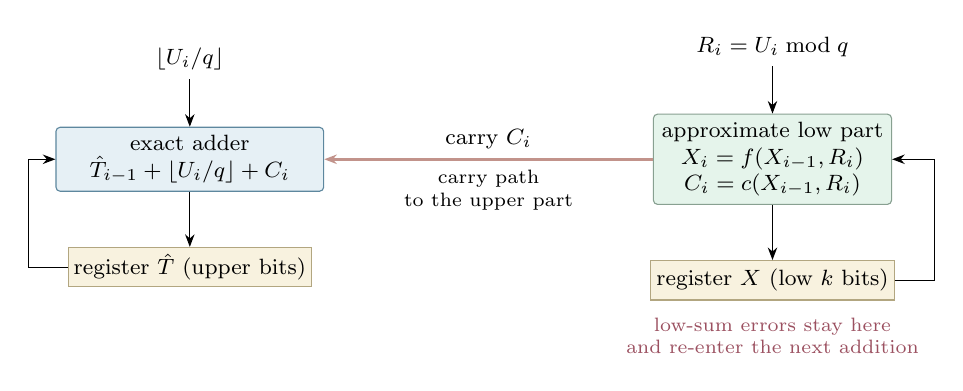
\begin{tikzpicture}[font=\footnotesize,>={Stealth[length=1.6mm]},
  box/.style={draw=paletteBlueEdge,fill=paletteBlueFill,rounded corners=1.5pt,align=center,minimum height=8mm,inner sep=3pt},
  reg/.style={draw=paletteYellowEdge,align=center,minimum height=5mm,minimum width=26mm,inner sep=2pt,fill=paletteYellowFill}]
\node[box,minimum width=34mm] (up) at (0,0) {exact adder\\$\hat T_{i-1}+\lfloor U_i/q\rfloor+C_i$};
\node[box,minimum width=30mm,fill=paletteMintFill,draw=paletteMintEdge] (lo) at (74mm,0) {approximate low part\\$X_i=f(X_{i-1},R_i)$\\$C_i=c(X_{i-1},R_i)$};
\node[reg,below=7mm of up] (hr) {register $\hat T$ (upper bits)};
\node[reg,below=7mm of lo] (xr) {register $X$ (low $k$ bits)};
\node[above=6mm of up] (uh) {$\lfloor U_i/q\rfloor$};
\node[above=6mm of lo] (u) {$R_i=U_i\bmod q$};
\draw[->] (uh) -- (up); \draw[->] (u) -- (lo);
\draw[->] (up) -- (hr); \draw[->] (lo) -- (xr);
\draw[->] (hr.west) -- ++(-5mm,0) |- (up.west);
\draw[->] (xr.east) -- ++(5mm,0) |- (lo.east);
\draw[->,draw=paletteCoralEdge,line width=1.1pt] (lo.west) -- node[above]{carry $C_i$} node[below,align=center]{\scriptsize carry path\\[-1pt]\scriptsize to the upper part} (up.east);
\node[below=1mm of xr,align=center,font=\scriptsize,text=paletteRoseText] {low-sum errors stay here\\and re-enter the next addition};
\end{tikzpicture}
\caption{Carry propagation in a split accumulator. Only the carry $C_i$
reaches the upper part; low-sum errors remain in the low register $X_i$
and enter the next addition.}
\label{fig:concept}
\end{figure}

\subsection{Carry conservation}

To isolate the source of accumulated error, we separate the carry sum from
the bounded content of the low register.
\begin{lemma}[Carry conservation]\label{lem:conservation}
For every input sequence,
\begin{equation}
E_n=\sum_{i=1}^n\bigl(qC_i-R_i\bigr)+\rho(X_n)-\rho(X_0).
\label{eq:conservation}
\end{equation}
\end{lemma}
\begin{proof}
$T_n-T_0=q(\hat T_n-\hat T_0)+\rho(X_n)-\rho(X_0)$ and
$q(\hat T_n-\hat T_0)=\sum_i(U_i-R_i)+q\sum_iC_i$.
Substituting the second expression into the first and subtracting
$\sum_iU_i$ gives Eq.~\eqref{eq:conservation}.
\end{proof}

For a lower-part adder, $|\rho(X_n)-\rho(X_0)|<q$, so the carry stream
determines accumulated error up to a bounded term (Fig.~\ref{fig:concept}).
An exact low part keeps $q\sum_iC_i-\sum_iR_i$ bounded, providing the
reference for judging an approximate low part.

Fig.~\ref{fig:carryidentity} checks the identity on three lower-part
designs. The measured error and the carry-based reconstruction coincide
at every step. The carry term alone differs by the bounded low-state
readout in Eq.~\eqref{eq:conservation}.

\begin{figure}[t]
\centering
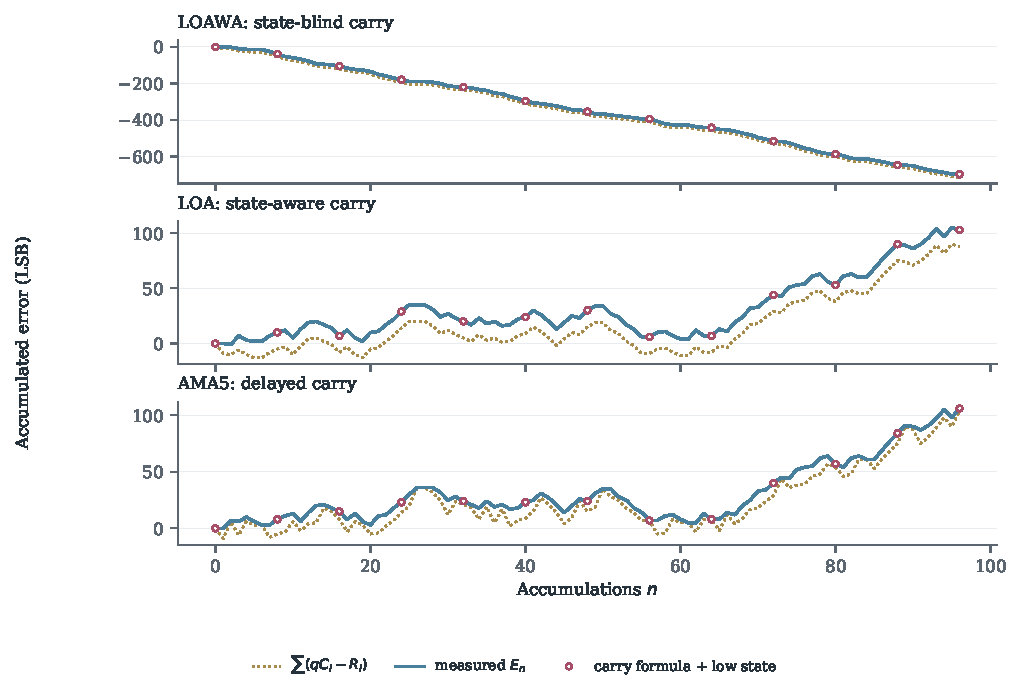
\includegraphics[width=\linewidth]{figures/carry_identity.pdf}
\caption{Measured and reconstructed accumulated error for LOAWA, LOA, and
AMA5 at $k=4$ on one sequence of 96 unsigned operands. Markers (carry sum
plus low-register term) coincide with the measured error at all 97 steps;
the dotted curve shows the carry sum alone.}
\label{fig:carryidentity}
\end{figure}

\subsection{State-blind carries}

If the carry ignores the low state, it can be computed from the fresh
operand before exact accumulation.
\begin{theorem}[Quantizer equivalence]\label{thm:blind}
Suppose $c(x,u)=g(u)$ for all states $x$. Let $Q(U)=U-R+q\,g(R)$ and let
$E'_n=\sum_{i=1}^n\bigl(Q(U_i)-U_i\bigr)$ be the error of an exact accumulator
of the quantized operands. Then for every input sequence and every $n$,
\begin{equation}
|E_n-E'_n|=|\rho(X_n)-\rho(X_0)|\le\max\rho-\min\rho\ (<q\text{ for a lower-part adder}).
\end{equation}
\end{theorem}
\begin{proof}
$E'_n=\sum_i(qg(R_i)-R_i)=\sum_i(qC_i-R_i)$.
Lemma~\ref{lem:conservation} then leaves only the difference between the
initial and final low-register readouts.
\end{proof}

We call the exact accumulator of $Q(U)$ the \emph{quantizer twin}.
The equivalence holds for correlated, nonuniform, and adversarial inputs;
whenever long-run drift and diffusion exist, they coincide for the design
and its twin.
Truncation ($g\equiv0$) is the twin of every design whose carry is
always zero (carry-cut).
Round-half-up ($g(u)=u_{k-1}$) is the twin of every design whose carry
copies the top bit of the fresh residue.

\begin{corollary}[Hardware]\label{cor:prune}
In a state-blind accumulator the upper register bits are functionally
independent of the low-state registers. Tying those registers to constants
and propagating the constants turns any netlist of the design, by removing or
simplifying cells only, into one whose upper outputs $T[W{-}1{:}k]$ equal
those of the quantizer twin.
\end{corollary}
\begin{proof}
By Eq.~\eqref{eq:split} the next upper value is
$\hat T_{i-1}+\lfloor U_i/q\rfloor+g(R_i)$, a function of the upper registers
and the operand only, so constants on the low-state registers leave the upper
next-state functions unchanged. When the fan-in cone of the upper registers
contains no low-state register, as in every netlist of Section~\ref{sec:hw},
extracting that cone yields the twin from a subset of the original cells.
\end{proof}

For uniform residues, the values $qg(r)-r$ are $q$ distinct integers.
It follows that $\Var(qg(R)-R)\ge(q^2-1)/12$, with equality for rounding and
truncation. A state-blind design cannot have smaller diffusion than
rounding at its own width.
For a nonuniform operand law, we need the best state-blind carry.
\begin{theorem}[Law-optimal state-blind design]\label{thm:threshold}
Let the residues be independent with an arbitrary law $p$ on $\Z_q$. Among
all integer carry functions $g$, the diffusion $\Var_p(qg(R)-R)$ is minimized
by a threshold quantizer $g(u)=g_0+\mathbf1\{u\ge\theta\}$ for some
$\theta\in\{0,\ldots,q\}$ and integer $g_0$, which affects only the drift.
\end{theorem}
\begin{proof}
Only residues in the support $U_p=\{u:p(u)>0\}$ affect the variance. Let
$v_u=qg(u)-u$ and $m=\E_p v_R$. If some $u\in U_p$ has $|v_u-m|>q/2$,
changing $g(u)$ by one moves $v_u$ by $q$ towards $m$ and strictly lowers
$\E_p(v_R-m)^2$, hence the variance. Up to a common shift of $g$, only
finitely many carry functions have variance below any given value, so
repeated moves stop, and a minimizer exists in which every $v_u$,
$u\in U_p$, lies in $[m-q/2,m+q/2]$. The two endpoints cannot both be
taken, because values $q$ apart would be congruent modulo $q$, whereas
$v_u\equiv-u$ are distinct. All values therefore lie in a half-open window
$[a,a+q)$, which fixes $g(u)=\lceil (a+u)/q\rceil$ on $U_p$. This formula is
nondecreasing in $u$ and takes two adjacent values on $\Z_q$, so it is a
threshold function. Using it also for residues outside $U_p$ leaves the
variance unchanged.
\end{proof}

A threshold quantizer from Theorem~\ref{thm:threshold} compares the fresh
residue with a fixed value and passes the result as a carry to the upper
part without a low register. No state-blind design can exploit the
operand law better. Under the product-residue laws of
Section~\ref{sec:hw},
its improvement
over round-half-up is at most 1.5\% in diffusion.

The lower-part OR adder has a state-aware carry, yet its accumulated
error stays close to that of rounding.
\begin{theorem}[LOA in an accumulator]\label{thm:loa}
For the lower-part OR adder, $z(x,u)=x\lor u$ and $c(x,u)=x_{k-1}\land u_{k-1}$.
Let $E'_n$ be the error of the round-half-up twin ($g(u)=u_{k-1}$). Then for
every initial state and every input sequence, $|E_n-E'_n|\le q$.
\end{theorem}
\begin{proof}
The state is the bitwise OR of $X_0$ and all residues so far, so its top bit
is zero up to the first time $\tau$ at which it or a residue has its top bit
set, and one afterwards. Before $\tau$ both carries are zero. At $\tau$ the
twin carries one more (only if $(X_0)_{k-1}=0$); after $\tau$,
$C_i=u_{k-1}=g(R_i)$. By Lemma~\ref{lem:conservation},
$E_n-E'_n=-q\,\mathbf1\{\tau\le n,\ (X_0)_{k-1}=0\}+X_n-X_0$, and
$0\le X_n-X_0\le q-1$.
\end{proof}

By Theorem~\ref{thm:loa}, LOA's OR gates and $k$ low registers do not
improve long-run accuracy.
AMA5~\cite{gupta2013ama}, with the state as left operand,
stores the fresh residue and emits its top bit one operation later.
Lemma~\ref{lem:conservation} shows that this delay leaves it within $q$
of round-half-up for every input (supplementary material).

\subsection{Exact drift, diffusion, and finite-length MSE}

From here on, the residues $R_i$ are independent with law $p$ on
$\Z_q$ (uniform unless stated). Then $X_i$ is a Markov chain with kernel
$P(x,y)=\sum_u p(u)\mathbf 1\{f(x,u)=y\}$. Define the reward
$Y(x,u)=qc(x,u)-u$ and its state mean
$\bar Y(x)=\sum_up(u)Y(x,u)$. Set
$A(x,y)=\sum_up(u)Y(x,u)\mathbf1\{f(x,u)=y\}$ and
$B(x,y)=\sum_up(u)Y(x,u)^2\mathbf1\{f(x,u)=y\}$.

To evaluate finite-length error under nonuniform laws, we compute its
moments from the finite-state model.
\begin{theorem}[Exact moments]\label{thm:moments}
With row vectors $v_0=\delta_{X_0}$, $m_0=s_0=0$ and
$v_i=v_{i-1}P$, $m_i=m_{i-1}P+v_{i-1}A$, $s_i=s_{i-1}P+2m_{i-1}A+v_{i-1}B$,
the sum $Y_1+\dots+Y_n$ has mean $m_n\mathbf1$ and second moment $s_n\mathbf1$,
and $E_n$ follows by adding $\rho(X_n)-\rho(X_0)$. If a single recurrent class
with stationary law $\pi$ is reachable from $X_0$, the drift is $\mu=\pi\bar Y$
and the diffusion is
\begin{equation}
\sigma^2_\infty=\sum_x\pi(x)\Var_{u\sim p}\bigl[Y(x,u)+\phi(f(x,u))\bigr],
\label{eq:diffusion}
\end{equation}
where $\phi$ solves the Poisson equation $\phi-P\phi=\bar Y-\mu$.
\end{theorem}
\begin{proof}
The recursion conditions on the state before each addition. For the
asymptotics, $D_i=Y_i-\mu+\phi(X_i)-\phi(X_{i-1})$ is a martingale difference,
and $\sum_iY_i-n\mu=\sum_iD_i-\phi(X_n)+\phi(X_0)$ with $\phi$ bounded, so
$\Var(E_n)/n\to\E_\pi[D^2]$. The Poisson equation is solvable on every
irreducible finite chain, periodic or not~\cite{kemeny1960,glynn1996poisson}.
\end{proof}

Every design studied here has one recurrent class reachable from the
cleared state. Consequently, $\E[E_n]=\mu n+O(1)$ and
$\Var(E_n)=\sigma^2_\infty n+O(1)$.
For a MAC cleared after a known $n$, setting the clear value to
$-\mathrm{round}(\E[E_n])$ instead of zero removes the mean error with a
constant in the clear logic. We use the resulting compensated MSE at $n$
as the primary quality metric, with diffusion giving its long-run rate.
We also express diffusion as the rounding-equivalent precision
$t_{\mathrm{eq}}=\tfrac12\log_2(12\sigma^2_\infty+1)$, the real-valued number
of rounded operand bits with the same diffusion.

\subsection{An information bound}
\label{sec:bound}

The low register retains information from each operand through its state
transitions. Let $p_{x}(y)$ be the probability of moving from state $x$ to
$y$. The entropy rate of the stationary chain is
$h=H(X_i\mid X_{i-1})=-\sum_x\pi(x)\sum_yp_x(y)\log_2p_x(y)$; it measures
new information stored per operation, while deterministic next states
have zero transition entropy.

Under uniform residues, Theorem~\ref{thm:bound} shows that diffusion
cannot fall below a floor set by the information the low register stores.
\begin{theorem}[Entropy bound]\label{thm:bound}
Let the residues be independent and uniform on $\Z_q$, and let a single
recurrent class be reachable. For any low-part machine,
\begin{equation}
\sigma^2_\infty\ \ge\ \frac{q^2\sum_x\pi(x)\sum_yp_x(y)^3-1}{12}
\ \ge\ \frac{q^2\,2^{-2h}-1}{12}
\ \ge\ \frac{(q/S)^2-1}{12},
\label{eq:bound}
\end{equation}
where $S$ is the largest number of distinct successors of a recurrent state.
For every integer $s\in\{0,\ldots,k\}$, all three bounds hold with equality
for exact accumulation of the operand rounded at $k-s$ bits, which keeps
$s=h=\log_2S$ exact low bits.
\end{theorem}
\begin{proof}
Fix $x$ and group the $q$ residues by successor $y$. Group $y$ has
$m_{xy}=q\,p_x(y)$ members. Inside the group the values
$Y(x,u)+\phi(y)=qc(x,u)-u+\phi(y)$ share the shift $\phi(y)$, and the integers
$qc(x,u)-u$ are distinct because their residues modulo $q$ are. A set of $m$
distinct integers has variance at least $(m^2-1)/12$. By the law of total
variance and Eq.~\eqref{eq:diffusion},
$\sigma^2_\infty\ge\sum_x\pi(x)\sum_yp_x(y)(m_{xy}^2-1)/12$, the first bound.
For the second, $\sum_yp_x(y)^3=2^{-2H_3(p_x)}$ with the R\'enyi entropy
$H_3\le H$~\cite{renyi1961}, and Jensen's inequality for the convex
$t\mapsto2^{-2t}$ gives $\sum_x\pi(x)2^{-2H(p_x)}\ge2^{-2h}$. The third
follows from $h\le\log_2S$. For rounding with $s$ kept bits every group is a
cyclic interval of $q/S$ consecutive residues with consecutive values, and
the groups have equal means.
\end{proof}

In rounding-equivalent bits the bound reads
\begin{equation}
k-t_{\mathrm{eq}}\ \le\ h\ \le\ \log_2S .
\label{eq:bits}
\end{equation}
Compared with dropping all $k$ bits, a low part gains at most its
state-transition entropy rate in accuracy bits. Exact accumulation of
rounded operands attains this at integer rates. The gain cannot exceed
the register count, and the entropy bound is sharper when the carry does not
use all stored information.

Equality in the entropy bound imposes a restriction on the state rate.
\begin{proposition}[Integer tightness]\label{prop:integer}
If the entropy bound in Eq.~\eqref{eq:bound} holds with equality, then $h$ is
an integer.
\end{proposition}
\begin{proof}
Equality requires $H_3(p_x)=H(p_x)$, i.e.\ $p_x$ uniform on a support of
$2^{j_x}$ elements (the masses are multiples of $1/q$), and, for Jensen's
inequality, $H(p_x)=j_x$ constant on the support of $\pi$.
\end{proof}


The $2^{-2h}$ form of Eq.~\eqref{eq:bound} mirrors the distortion--rate
law $q^22^{-2R}/12$ of uniform scalar quantization~\cite{gray1998quant},
with the stored entropy rate taking the place of the coding rate. The bound
needs uniform residues: a one-bit low part exactly accumulates residues
taking only the values $0$ and $q/2$. The grouping argument extends to
any law.

For nonuniform residues, transition groups and their probabilities give a
machine-specific bound.
\begin{theorem}[Law-dependent bound]\label{thm:lawbound}
Let the residues be independent with law $p$ and a single recurrent class be
reachable. For a state $x$ and successor $y$, let $G_{xy}$ be the residues
leading from $x$ to $y$, and let $V^\ast(G_{xy})$ be the least $p$-weighted
variance of integers $v_u\equiv-u\pmod q$, $u\in G_{xy}$. Then
\begin{equation}
\sigma^2_\infty\ \ge\ \sum_x\pi(x)\sum_y p(G_{xy})\,V^\ast(G_{xy}),
\label{eq:lawbound}
\end{equation}
and $V^\ast(G)$ is the minimum over the $q$ cyclic cuts of $G$.
\end{theorem}
\begin{proof}
Condition on the current state and group the input residues by their
successor state, as in the proof of Theorem~\ref{thm:bound}. Within each
group the Poisson correction is constant, so its conditional variance is
at least $V^\ast(G_{xy})$. Weighting this inequality by the probability of
each transition and by the stationary state probability gives
Eq.~\eqref{eq:lawbound}. The window argument of
Theorem~\ref{thm:threshold} reduces each group minimum to a cyclic cut.
\end{proof}

For uniform $p$ and consecutive groups, this reduces to the first
inequality of Eq.~\eqref{eq:bound}. The machine-specific bound limits
how close a given low part can come to exact accumulation under its
operand law. Under the product-residue laws of Section~\ref{sec:hw}, it holds
for all 226 design--law pairs and is tight for 11. The supplementary
material reports randomized property tests of all bounds on several
thousand machines and laws.

\section{Census of published designs}
\label{sec:census}

The census covers unsigned EvoApproxLib v2022 adders whose residue
property is proved by exhaustive enumeration or SAT, as described in
Section~\ref{sec:model}. Identifiers such as \texttt{add8u\_2LL} are the
library's official cell names: \texttt{add8u} denotes an 8-bit unsigned
adder, and the suffix identifies the catalog entry. The census also
covers five classic families at
$k=2,\ldots,8$: LOA, LOAWA, ETA-I, AMA2, and AMA5. Each classic cell is
rippled over $k$ bits~\cite{gupta2013ama}. All 30 approximate 8-bit
cells qualify. Among the 12-bit cells, 16 of 28 have a SAT-proved
residue width $k\le8$. Among the 16-bit cells, 8 of 30 qualify.

Table~\ref{tab:census} summarizes exact metrics with the accumulator
state as the left operand. Fig.~\ref{fig:statebits} shows accuracy gain
against the state entropy rate. We keep the same operand orientation
in the hardware synthesis of Section~\ref{sec:hw}. We checked the
values by simulating wide accumulators on uniform, skewed, constant,
ramp, and random-walk streams.

\begin{table}[t]
\centering
\caption{Several state-aware designs store no new information.
The census uses the accumulator state as the
left operand. ``Blind'' counts designs whose carry is independent of state
(Theorem~\ref{thm:blind}), while $h{=}0$ counts designs that store no new
information. ``Tight'' counts designs whose diffusion equals the entropy
bound of Theorem~\ref{thm:bound}, including the trivial $h=0$ cases. ``Gain''
is the maximum $k-t_{\mathrm{eq}}$ in bits. The last columns give the median
and maximum accuracy gain per bit of entropy rate among state-aware designs
with $h>0$.}
\label{tab:census}
\small
\setlength{\tabcolsep}{4pt}
\begin{tabular}{lrrrrrrrr}
\toprule
Source & $n$ & $k$ & Blind & $h{=}0$ & Tight & Max gain & \multicolumn{2}{c}{Efficiency}\\
 & & & & & & & med. & max.\\
\midrule
EvoApproxLib 8-bit  & 30 & 1--8 & 15 & 5 & 6 & 3.91 & 0.32 & 1.00\\
EvoApproxLib 12-bit & 16 & 1--8 & 8 & 2 & 3 & 2.00 & 0.14 & 1.00\\
EvoApproxLib 16-bit & 8  & 2--7 & 3 & 1 & 1 & 0.75 & 0.00 & 0.28\\
LOA~\cite{mahdiani2010loa}       & 7 & 2--8 & 0 & 7 & 7 & 0.00 & -- & --\\
LOAWA~\cite{albicocco2012loawa}  & 7 & 2--8 & 7 & 7 & 7 & 0.00 & -- & --\\
ETA-I~\cite{zhu2010eta}          & 7 & 2--8 & 7 & 7 & 7 & 0.00 & -- & --\\
AMA5~\cite{gupta2013ama}         & 7 & 2--8 & 0 & 0 & 0 & 0.00 & 0.00 & 0.00\\
AMA2~\cite{gupta2013ama}         & 7 & 2--8 & 0 & 0 & 0 & 0.33 & 0.09 & 0.32\\
\bottomrule
\end{tabular}
\end{table}

\begin{figure}[t]
\centering
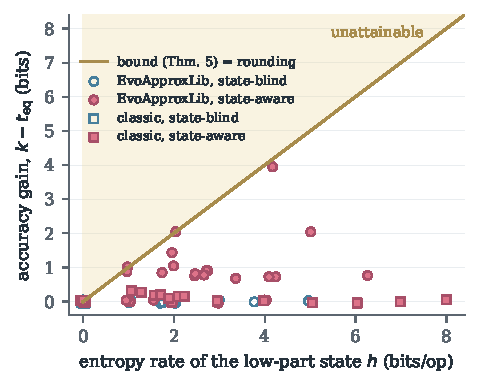
\includegraphics[width=0.62\linewidth]{figures/state_bits.pdf}
\caption{Accuracy gain versus low-state entropy rate for the 89 designs.
The entropy bound (Theorem~\ref{thm:bound}) excludes the shaded region;
rounding lies on the diagonal.}
\label{fig:statebits}
\end{figure}

Table~\ref{tab:census} identifies 26 of 54 library cells, plus LOAWA and
ETA-I, as state-blind. Their upper results match truncation or rounding
despite additional low-part logic. Swapping operands changes the class
of 13 cells; in at least one orientation, 33 are state-blind, so operand
orientation can make low-part logic removable.

LOA has a state-aware carry but retains no information over long
sequences, whereas AMA5 delays rounding by one operation. Neither improves
accuracy over its rounding twin, and together their 14 variants reduce
to rounding.

State-aware cells differ in how much of the entropy bound they attain.
\texttt{add8u\_02Y} and \texttt{add12u\_0AZ} meet the bound, while
\texttt{add8u\_6S4} and \texttt{add8u\_6SM} reach 93\% and 94\% of it.
The median 8-bit state-aware cell gains only 0.32 bits per bit of entropy
rate. \texttt{add8u\_3RE} has 128 recurrent states but gains only
2 bits, showing that state count alone is insufficient.

Drift changes the ranking of designs: after optimal constant compensation,
single-addition MSE predicts accumulated MSE at $n=256$ well (Kendall
$\tau=0.90$--$1.00$). Without compensation, $\tau$ falls to 0.36--0.57.
Among 434 ordered 8-bit pairs, 99 reverse their ranking. For example,
\texttt{add8u\_4M7} has mean single-addition error $-0.5$ but accumulated
drift $-3.5$ per operation.

\section{Hardware evaluation}
\label{sec:hw}

\subsection{Experimental setup}

We evaluate each design as a 24-bit accumulator with a 16-bit operand
and synchronous clear, as in a MAC unit. We zero-extend unsigned
products and sign-extend two's-complement products. The baselines
include the full exact accumulator. At $t=1,\ldots,8$, they also
include exact accumulation of operands rounded half-up, truncated,
or truncated with a carry-in of one.
Here \texttt{round\_$t$} and \texttt{trunc\_$t$} denote exact accumulation
of operands rounded half-up or truncated at $t$ bits, respectively.
Throughout this section, a reference is an exact accumulator of rounded
or truncated operands.
These references retain only the upper $24-t$ register bits. For an
approximate design, we connect the published lower-part adder RTL to an
exact adder for bits $k$ and above. The cell receives zeroed high
operand bits, giving
$z=o[k{-}1{:}0]$ and $c=o[k]$ as in Lemma~\ref{lem:carry}, yielding
89 approximate and 25 reference accumulators for each operand variant
(unsigned or signed products).

Yosys~\cite{wolf_yosys} elaborates the RTL, which ABC~\cite{brayton2010abc}
maps each design to X1 cells of the Nangate45 typical
library~\cite{nangate45}. Three structural pre-optimizations and
six delay-relaxation settings of ABC's delay-driven \texttt{\&nf} mapper
produce 18 netlists per design. ABC's combinational equivalence checker
\texttt{cec} proves each mapped netlist
equivalent to its RTL, with registers matched by name. We also compare
each netlist with the reference model of Eq.~\eqref{eq:split} on a
4000-operation MAC trace. All $2\times115\times18$ netlists passed both
checks. The 115 designs per variant comprise the 114 accumulators above
and the exact library cell \texttt{add8u\_1HG}.

Reported area includes registers; reported delay is ABC's
register-to-register delay. We estimate energy per accumulation with
a unit-delay simulation. It counts glitches and uses Liberty pin
capacitances and internal-energy tables. The inputs are products of
uniform 8-bit unsigned or signed operands. We call the distribution of
the low $k$ bits of these products the product-residue law.

\paragraph{Post-route flow}
We also place and route every design with OpenROAD-flow-scripts and its
Nangate45 platform~\cite{ajayi2019openroad}. OpenROAD-flow-scripts (ORFS)
runs synthesis,
floorplanning at fixed core utilization, global and detailed placement,
clock-tree synthesis, timing repair, global and detailed routing, and
parasitic extraction. The accumulator ports are unbuffered because they
are internal MAC nets; we route each design at a relaxed clock of
1.5~ns and a tight clock of 0.55~ns. The latter is the fastest period
at which the exact accumulator closes timing. We use four
implementation configurations: the default, area-oriented ABC mapping,
and core utilizations of 40\% and 65\%. As in the synthesis study,
a design's cost is its best routed result
with nonnegative setup slack. Post-route standard-cell area includes clock
and repair buffers but excludes fill and tap cells. We simulate every routed
netlist at gate level on 2000 MAC products, checking its outputs against
the reference model at each cycle.
OpenSTA computes post-route power from the simulation's switching
activity and extracted parasitics. All 2480 routed accumulator
netlists passed the cycle check. We call variation across mapping or
routing configurations implementation scatter.

\paragraph{FPGA flow}
Vivado 2022.2 implements every signed accumulator out of context on the
KV260 device (\texttt{xck26}), testing a different implementation
technology. The flow runs synthesis, placement, and routing at a 2~ns
clock. We report routed configurable logic block (CLB) LUTs and
registers. On this device, exact
adders map to dedicated carry chains; approximate low parts use LUTs.

\subsection{Dominance of state-blind designs}
\label{sec:blindhw}

State-blind carries make the low registers unnecessary
(Corollary~\ref{cor:prune}). We tested this by extracting the fan-in
cone of the upper registers from each of the 720 mapped netlists.
These netlists cover the 40 state-blind designs for each operand
variant, and no cone contained a low register. ABC \texttt{cec} proved
every extracted netlist equivalent to the RTL of its quantizer twin,
giving 1440 proofs in total.

Extraction never increased area, delay, or energy relative to the original
netlist. Area fell by up to 29.4\%. The medians were 8.8\% for unsigned
operands and 7.8\% for signed operands. Energy fell by up to 25.7\%.
The removable logic follows from the circuit structure regardless of
the mapping heuristic. We also routed the pruned RTL under all eight
clock and configuration settings, tying low-state reads to zero.
Every routed netlist matched the twin model at each cycle. Its best
area was a median 5--8\% below that of the unpruned design.
We count pruned netlists, like rounding and truncation, as
implementations of the quantizer twins.

\subsection{All designs}

\begin{figure}[t]
\centering
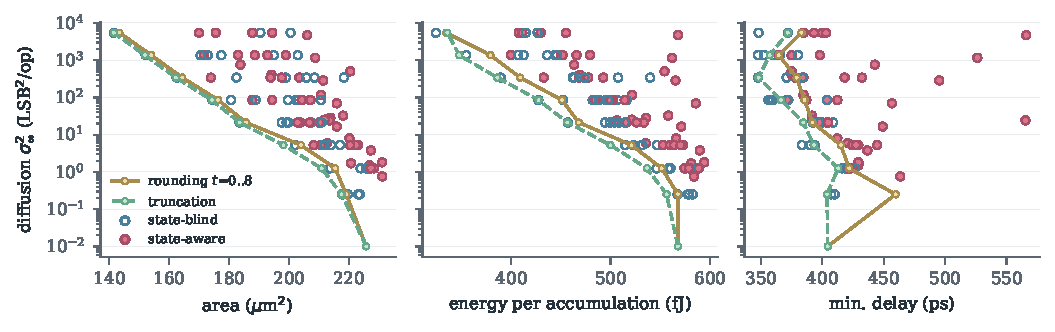
\includegraphics[width=\linewidth]{figures/hw_pareto.pdf}
\caption{Area, energy, and delay versus diffusion for the 89 unsigned
designs under uniform residues. Lines denote exact accumulation of rounded
and truncated operands, which set the lower cost envelope.}
\label{fig:hw}
\end{figure}

\begin{figure}[t]
\centering
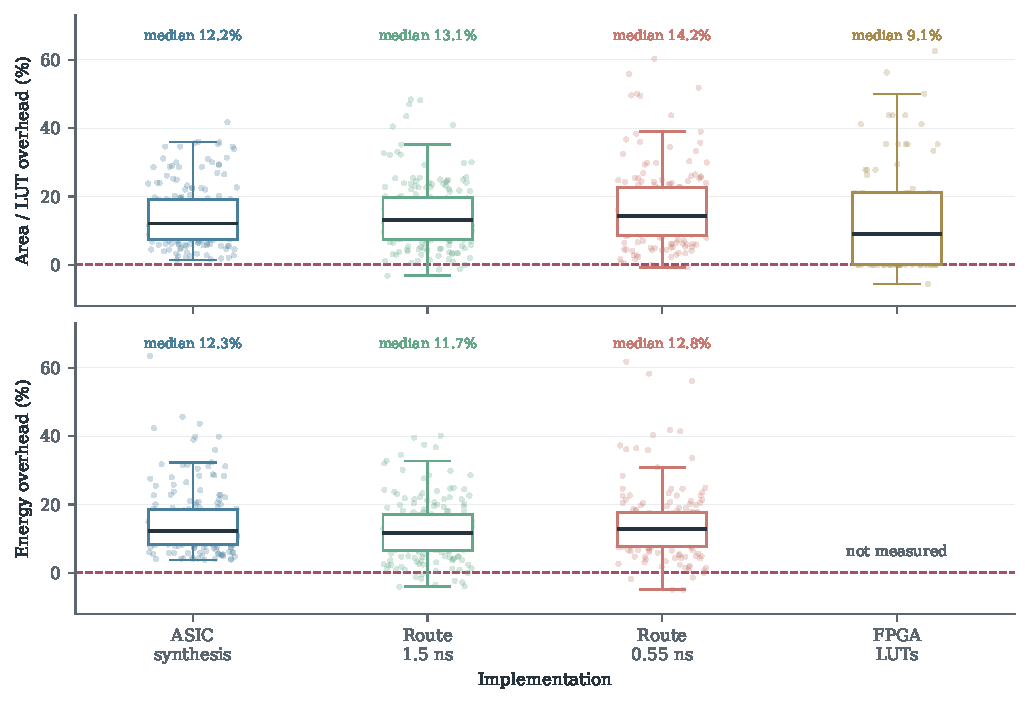
\includegraphics[width=\linewidth]{figures/cost_distribution.pdf}
\caption{Cost differences from the cheapest equally accurate reference
under the product-residue law; zero denotes equal cost. FPGA values are
LUT-count differences, and FPGA energy was not measured.}
\label{fig:costdist}
\end{figure}

\begin{table}[t]
\centering
\caption{Area and energy penalties relative to the cheapest exact reference
accumulator with no larger diffusion under the product-residue law.
Entries are medians over designs, with minima in parentheses; a negative
minimum means that at least one design was cheaper than every equally
accurate reference. Synthesis takes the best of 18 mappings. Post-route
takes the best of four routed configurations that meet the clock and counts
the routed pruned netlists of Section~\ref{sec:blindhw} as twin
implementations; without
them, the post-route medians are 7--16\%. Under the uniform law,
post-route medians reach 19\% (Table~S2).}
\label{tab:hw}
\footnotesize
\setlength{\tabcolsep}{3pt}
\begin{tabular}{llrrrr}
\toprule
 & & \multicolumn{2}{c}{Unsigned} & \multicolumn{2}{c}{Signed}\\
\cmidrule(lr){3-4}\cmidrule(lr){5-6}
Flow & Class & Area (\%) & Energy (\%) & Area (\%) & Energy (\%)\\
\midrule
Synthesis & blind (40) & 11.5 (1.4) & 10.8 (3.9) & 9.5 (1.9) & 11.1 (3.8)\\
          & aware (49) & 13.7 (2.1) & 14.6 (4.1) & 12.2 (1.7) & 12.6 (4.1)\\
Routed, 1.5 ns & blind & 14.1 ($-1.4$) & 9.2 ($-3.5$) & 10.2 (0.6) & 13.3 (0.5)\\
               & aware & 13.5 ($-1.3$) & 9.9 ($-4.1$) & 11.7 ($-3.2$) & 13.9 ($-3.9$)\\
Routed, 0.55 ns & blind & 13.5 ($-0.7$) & 10.9 ($-4.9$) & 11.1 (2.4) & 11.8 (2.4)\\
                & aware & 17.1 (0.5) & 13.9 ($-1.4$) & 15.7 (1.6) & 15.4 ($-1.8$)\\
\bottomrule
\end{tabular}
\end{table}

The hardware comparisons give the same ordering across quality metrics.
Fig.~\ref{fig:hw} relates hardware metrics to diffusion under uniform
residues. Fig.~\ref{fig:costdist} shows the cost distribution by flow under
the product-residue law. Table~\ref{tab:hw} compares designs with references under
the product-residue law. Uniform-law diffusion and
compensated MSE give the same conclusions at $n=144$ and $576$.
Differences below 1\% count as ties (supplementary material).

\paragraph{Synthesis}
References lead every approximate design in synthesized area or
energy at matched accuracy. None of the 89 approximate designs matches
the best area or energy under any evaluated law, metric, or operand
type. This remains true without registers for 87 designs.
References jointly dominate every state-blind mapped point in area,
delay, and energy. Only 6 unsigned and 11 signed state-aware points
escape joint dominance among 1602 points. The exact upper chain
usually sets the critical path, and approximate low parts are a median
2--8\% slower than equally accurate references.
At a common delay constraint, three signed designs each have one
point with lower area and energy than every reference meeting that
constraint: \texttt{add8u\_2LL}, \texttt{add8u\_2J3}, and
\texttt{add12u\_0C9}. These advantages coincide with a 4\% difference
between fastest mappings (within implementation scatter; supplementary
material).

\paragraph{After routing}
Median area and energy penalties remain at 9--19\% after placement,
routing, and timing repair. They are 7--16\% when pruned netlists are
excluded from the reference set. The median within-design routed-area
range across four configurations is 19--21\% (Supplementary material,
Implementation scatter). Each reported design cost is the best of four
routed configurations, and the reported penalty is a median across 89
designs rather than one implementation's scatter.

LOA and AMA5, both pathwise within $q$ of \texttt{round\_$k$},
reach differences of $-2.6\%$ in area and $-8.4\%$ in energy against their
own rounding twins (supplementary material, Implementation scatter).
This pairwise comparison differs from the comparison with the cheapest
reference of no larger diffusion used in Table~\ref{tab:hw} and the
abstract. These negative minima are comparable
to implementation scatter; for state-blind designs, they cannot represent
an intrinsic advantage: Corollary~\ref{cor:prune} builds a twin by removing
cells from the design's own netlist.

Two state-aware designs are cheaper in both area and energy under
the product-residue law at 1.5~ns. For signed products, \texttt{add12u\_4NT}
saves 3.2\% in area and 3.9\% in energy. For unsigned products, LOA with
$k=2$ saves 1.3\% in area and 2.8\% in energy. LOA is pathwise within $q$
of \texttt{round\_2} (Theorem~\ref{thm:loa}), so the margin reflects
implementation scatter. Neither
design is cheaper under the uniform law or at 0.55~ns, while some other
state-aware designs save up to 4.1\% in energy but not in area.
At 0.55~ns every reference closes timing in at least one configuration;
four AMA2 variants, \texttt{add8u\_6S4}, and \texttt{add8u\_6SM} do not
close timing for at least one operand type.

\paragraph{FPGA}
Approximate designs generally use more FPGA resources at matched
accuracy. On the KV260, the median design uses one to two more LUTs
than the cheapest equally accurate reference. Against rounding and
truncation alone, ten designs save one LUT. Each needs one to five
more registers, so none uses fewer of both. With pruned twins counted
as references, only \texttt{add8u\_3RE} saves one LUT under the product
law, but it costs five more registers.

\paragraph{MAC context}
Rounding saves more area than the approximate cells in the routed
MAC comparison. In a registered $8\times8$ signed MAC, the exact
accumulator accounts for 46\% of cell area. Rounding products by
seven bits reduces MAC area by 16\%; eight bits reduces it by 18\%.
The approximate cells evaluated in Section~\ref{sec:cnn} reduce
area by 5--12\%. In this single-configuration comparison, LOA and
\texttt{add8u\_0E2} are 5--7\% larger than their twins.
\texttt{add8u\_2LL} matches \texttt{round\_5} within 0.2\%, while
the state-blind \texttt{add8u\_6QU} is 3.2\% smaller than
\texttt{trunc\_4} (within implementation scatter).
Corollary~\ref{cor:prune} yields a twin implementation from
\texttt{add8u\_6QU}'s own cells.

\section{Application: INT8 ResNet-20}
\label{sec:cnn}

We trained ResNet-20~\cite{he2016resnet} on
CIFAR-10~\cite{krizhevsky2009cifar} to 91.58\% top-1 accuracy.
We then folded batch normalization and quantized weights per channel
and activations per tensor to symmetric INT8~\cite{jacob2018quant}.
Each convolution and the classifier serially accumulate $L=27$ to
$576$ signed products in a 24-bit register.

Bit-exact simulation uses each design's $(z,c)$ table to evaluate 17
rounding and truncation references and 18 approximate designs. We compare
three settings: no compensation, a preload from uniform-law drift
$-\mathrm{round}(L\mu)$, and a data-calibrated preload
$-\mathrm{round}(\E E_L)$. For the last case, we use
Theorem~\ref{thm:moments} and the layer's product-residue law measured on 40
calibration images.

\paragraph{Exact metrics and equivalences on real data}
Product residues differ substantially from a uniform law: their total
variation distance from uniform modulo 256 is 0.27--0.92, partly
because ReLU produces many zeros. With each measured law,
Theorem~\ref{thm:moments} predicts accumulated MSE for 494
layer--design pairs. The median predicted-to-measured ratio is 0.978;
its interquartile range is 0.961--0.989. A uniform-law prediction
errs by a median factor of 3.4 in either direction, and drift dominates
these uncompensated errors. As the replication below
shows, the variance prediction must be conditioned on the number of
nonzero products.

State-blind designs and LOA closely match their quantizer twins in
test-image top-1 predictions. Table~\ref{tab:cnn} gives agreement of
98.9--99.9\%, as expected from the pathwise
Theorems~\ref{thm:blind} and~\ref{thm:loa}. Bounded low-register
readout flips the remaining near-ties. The \texttt{add8u\_0TP}
cell combines truncation with a constant carry; without compensation,
its accuracy falls to 25.3\%. After calibration, it agrees with
\texttt{trunc\_5} on 99.5\% of images.

\begin{table}[t]
\centering
\caption{Calibration restores accuracy for most designs. Top-1
accuracy (\%) and best signed-accumulator area are reported for
INT8 ResNet-20 on 1000 CIFAR-10 test images. The accuracy columns report no
compensation, uniform-law compensation for references, and data-calibrated
compensation (Cal.). ``--'' means not evaluated. Area is synthesized area.
``Twin'' is the share of predictions identical to the
calibrated quantizer twin. Exact INT8 accuracy is 92.3\%, and float accuracy
is 92.6\%.}
\label{tab:cnn}
\footnotesize
\setlength{\tabcolsep}{4pt}
\begin{tabular}{lrrrrrl}
\toprule
Design & None & Uniform & Cal. & Area ($\mu$m$^2$) & Twin & Twin ref. \\
\midrule
exact            & 92.3 & 92.3 & 92.3 & 254.8 &  & \\
\texttt{round\_4} & 92.3 & 92.6 & 92.6 & 212.8 &  & \\
\texttt{round\_6} & 92.5 & 92.4 & 92.8 & 195.5 &  & \\
\texttt{round\_7} & --   & 92.2 & 92.4 & 183.8 &  & \\
\texttt{trunc\_4} & 91.3 & 90.2 & 92.5 & 210.9 &  & \\
\texttt{trunc\_6} & 51.1 & 44.7 & 92.1 & 189.4 &  & \\
\texttt{trunc\_7} & --   & --   & 90.2 & 180.3 &  & \\
\midrule
\texttt{add8u\_6QU} (blind)  & 91.1 & -- & 92.2 & 228.5 & 99.2 & \texttt{trunc\_4}\\
\texttt{add8u\_0E2} (blind)  & 92.2 & -- & 92.1 & 199.5 & 99.0 & \texttt{round\_7}\\
\texttt{add8u\_0TP} (blind)  & 25.3 & -- & 92.1 & 214.1 & 99.5 & \texttt{trunc\_5}\\
ETA-I, $k{=}5$ (blind)       & 88.0 & -- & 92.0 & 236.5 & 99.5 & \texttt{trunc\_5}\\
LOA, $k{=}5$                 & 92.1 & -- & 92.3 & 241.8 & 99.9 & \texttt{round\_5}\\
\texttt{add8u\_6SM} (aware)  & 92.0 & -- & 92.6 & 241.5 & & \\
\texttt{add8u\_2LL} (aware)  & 92.1 & -- & 92.4 & 216.0 & & \\
\texttt{add8u\_0PL} (aware)  & 77.1 & -- & 92.1 & 224.2 & & \\
\texttt{add8u\_6S4} (aware)  & --   & -- & 92.4 & 240.2 & & \\
\bottomrule
\end{tabular}
\end{table}

\begin{figure}[t]
\centering
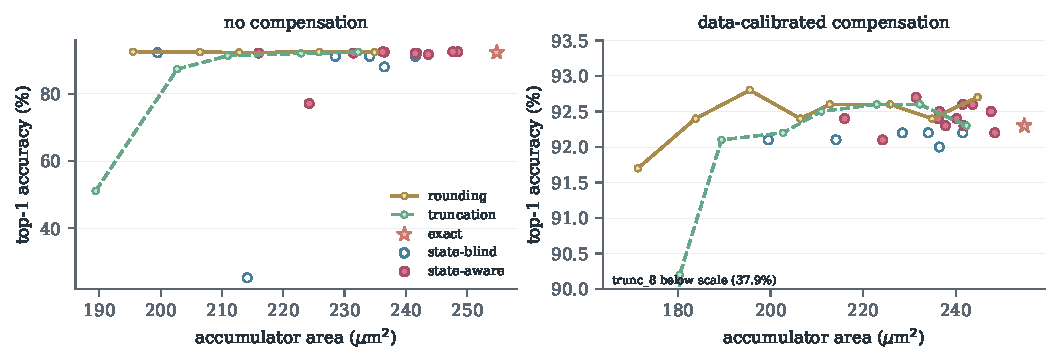
\includegraphics[width=\linewidth]{figures/cnn_accuracy.pdf}
\caption{ResNet-20 accuracy versus accumulator area without (left) and
with (right) calibrated compensation. Lines denote exact accumulation of
rounded and truncated products.}
\label{fig:cnn}
\end{figure}

\paragraph{Compensation and the cheapest equivalent accumulator}
Drift dominates inference accuracy without compensation
(Fig.~\ref{fig:cnn}). Truncating six bits reduces accuracy to 51.1\%.
Carry-cut designs follow their quantizer twins, while rounding remains at
92.3--92.5\%. A preload computed from uniform residues worsens
truncation to 44.7\% because it overcorrects residues concentrated
near zero.

Data-calibrated compensation restores most designs to 92.0--92.8\%
(Fig.~\ref{fig:cnn}), including low parts of up to eight bits.
The exceptions are \texttt{round\_8}, \texttt{trunc\_7}, and
\texttt{trunc\_8}. A second seed gives the same pattern for eleven
representative designs (supplementary material).

Layer requantization hides many calibrated low-bit errors by discarding
at least 7.4 accumulator least significant bits per channel.
To identify the smallest equivalent accumulator, we use all 10{,}000 test
images with a $\pm1$-point margin and a paired two one-sided test at
level 0.05. The comparison includes the exact accumulator
(91.46\%),
\texttt{round\_5}--\texttt{round\_8}, \texttt{trunc\_4}, \texttt{trunc\_6},
\texttt{trunc\_7}, three library cells, and LOA. The analysis sequence is
described with the replication below (supplementary material).

Most tested designs meet the one-point criterion; the exception is
\texttt{trunc\_7}, whose difference is $-1.92$ points.
The approximate cells remain within 0.12 points of exact.
\texttt{round\_8} loses 0.54 points with a 90\% interval of
$[-0.78,-0.30]$. Its synthesized area is 33\% lower and its routed
area is 40\% lower than exact (areas in Table~\ref{tab:cifar100}).
Equivalence fails with a half-point margin
(supplementary material). Under the stated criterion, \texttt{round\_8} is
the cheapest equivalent accumulator and accumulates rounded products
exactly. Among the evaluated approximate accumulators,
\texttt{add8u\_0E2} has the lowest area. It is the quantizer twin of
\texttt{round\_7} but is larger than \texttt{round\_7}.

Energy on the network's own operand stream gives the same ordering.
We re-simulated every mapped signed netlist on 10{,}080 real products
from two layers. Each of the 89 approximate designs used more energy
than the best reference with no larger diffusion, with a minimum penalty
of $+4.4\%$. The state-blind median was $+14.3\%$; the state-aware
median was $+15.9\%$. Rounding products by seven or eight bits would
also permit a
truncated multiplier~\cite{petra2010trunc}.

\paragraph{Protocol-fixed replication on CIFAR-100}
The margin and the 10{,}000-image run were chosen after the initial
1000-image analysis. We fixed a replication protocol before training
the second network; the protocol and its SHA-256 hash are included in the
public artifact (Data availability).
A ResNet-20 trained on CIFAR-100~\cite{krizhevsky2009cifar} with the
same recipe reaches 67.5\% float accuracy and 67.35\% exact INT8
top-1 accuracy. Quantization, accumulation, calibration,
and the twelve CIFAR-10 designs are unchanged, and we use all 10{,}000
test images. The
protocol states four hypotheses: H1, each of \texttt{add8u\_0E2},
\texttt{add8u\_6QU}, and LOA agrees with its quantizer twin on at least
98\% of predictions; H2, the median predicted-to-measured MSE ratio over
layer--design pairs lies in $[0.9,1.1]$; H3, paired equivalence with exact
at a one-point margin; and H4, no equivalent approximate low part has less
synthesized or routed area than the cheapest equivalent reference.
Table~\ref{tab:cifar100} reports the four prespecified outcomes.

\begin{table}[t]
\centering
\caption{Protocol-fixed CIFAR-100 replication on 10{,}000 test images with
data-calibrated compensation. $\Delta$ is the paired top-1 difference from
exact INT8 (67.35\%) in points with its 90\% interval; $\checkmark$ marks
equivalence at the one-point margin. Areas are the best signed synthesis
area and the best routed area at 1.5~ns ($\mu$m$^2$). ``Twin'' is the
share of predictions identical to the quantizer twin.}
\label{tab:cifar100}
\footnotesize
\setlength{\tabcolsep}{3pt}
\begin{tabular}{lrrcrrr}
\toprule
Design & Top-1 & $\Delta$ (90\% CI) & Eq. & Synth. & Routed & Twin\\
\midrule
exact             & 67.35 & 0                  & \checkmark & 254.8 & 421.9 & \\
\texttt{round\_5} & 67.34 & $-0.01$ $[-0.20,0.18]$ & \checkmark & 206.4 & 298.2 & \\
\texttt{round\_6} & 67.22 & $-0.13$ $[-0.37,0.11]$ & \checkmark & 195.5 & 306.4 & \\
\texttt{round\_7} & 67.43 & $+0.08$ $[-0.23,0.39]$ & \checkmark & 183.8 & 282.2 & \\
\texttt{round\_8} & 65.78 & $-1.57$ $[-2.02,-1.12]$ &          & 171.3 & 254.0 & \\
\texttt{trunc\_4} & 67.46 & $+0.11$ $[-0.12,0.34]$ & \checkmark & 210.9 & 365.0 & \\
\texttt{trunc\_6} & 65.96 & $-1.39$ $[-1.84,-0.94]$ &          & 189.4 & 304.3 & \\
\texttt{trunc\_7} & 58.97 & $-8.38$ $[-9.03,-7.73]$ &          & 180.3 & 264.4 & \\
\midrule
\texttt{add8u\_0E2} & 67.21 & $-0.14$ $[-0.46,0.18]$ & \checkmark & 199.5 & 282.5 & 95.0\\
\texttt{add8u\_6QU} & 67.58 & $+0.23$ $[0.00,0.46]$  & \checkmark & 228.5 & 334.9 & 98.1\\
\texttt{add8u\_2LL} & 67.32 & $-0.03$ $[-0.22,0.16]$ & \checkmark & 216.0 & 307.8 & \\
LOA, $k{=}5$        & 67.38 & $+0.03$ $[-0.16,0.22]$ & \checkmark & 241.8 & 326.9 & 97.9\\
\bottomrule
\end{tabular}
\end{table}

The cost ordering (H4) holds. Eight designs besides exact are
equivalent to it at the one-point margin and also at half a point.
\texttt{round\_8} is not equivalent, making \texttt{round\_7} the cheapest
equivalent accumulator, with 28\% less synthesized area
and 33\% less routed area than exact. Its quantizer twin
\texttt{add8u\_0E2} is 8.5\% larger after synthesis and 0.1\%
larger after routing, consistent with
Theorem~\ref{thm:blind}: the cell is a prunable twin of
\texttt{round\_7}. The other equivalent approximate designs are
9--19\% larger after routing. Tolerable rounding depth depends on
the task: eight bits for CIFAR-10 and seven for CIFAR-100.

Twin agreement fell below the 98\% threshold for two of the three
designs because near-ties are more frequent with 100 classes; H1 was
not met. The threshold came from CIFAR-10, where any two of the twelve
designs agree on at least 97.1\% of images. Even \texttt{round\_5} and
exact agree on 97.4\% of images in the replication.
For each of the three designs, its twin remains the reference with
the highest agreement. The pathwise bounds of
Theorems~\ref{thm:blind} and~\ref{thm:loa} still hold.

H2 was not met: the median ratio is 0.88, with an interquartile range
of 0.29--0.95. The variance prediction must be conditioned on the
number $N$ of nonzero products because calibrated compensation removes most
drift, leaving variance to dominate measured MSE; the uncompensated
validation above did not test this variance. A post hoc analysis
outside the protocol locates the gap: the median variance ratio is 0.94--0.99 for
rounding-type designs and 0.20--0.25 for truncation-type designs on
both CIFAR-10 and CIFAR-100. ReLU zeros make the number $N$ of nonzero
products per output vary across positions and images. A design with
nonzero mean per-operation error $\mu$ gains an extra variance
$\mathrm{Var}(N)\mu^2$. Applying Theorem~\ref{thm:moments}
conditionally on $N$, with the law of nonzero residues, gives
variance ratios of 0.95--1.04 for \texttt{trunc\_4},
\texttt{trunc\_6}, and \texttt{round\_5} on both datasets.
The independence assumption of Theorem~\ref{thm:moments} must
include the number of nonzero operands. The pathwise results and
hardware comparison do not use this assumption.

\paragraph{A workload without requantization headroom}
The FIR experiment retains the full accumulator output. We apply a
windowed-sinc low-pass filter with signed 8-bit taps to grayscale
Kodak images, using $L=64$ and $256$. Images 1--12 provide the
residue law and each design's compensation constant. Another 20{,}000
windows from images 13--24 provide output SNR measurements.
They span 32--80~dB, with 95\% bootstrap intervals.

Measured FIR outputs closely match their quantizer twins. At $L=256$,
\texttt{add8u\_6QU}, LOAWA, and ETA-I with $k=4$ reach 52.22~dB.
\texttt{trunc\_4} reaches 52.24~dB. LOA reaches 49.08~dB;
\texttt{round\_5} reaches 49.09~dB. AMA5 gives exactly the
54.80~dB of \texttt{round\_4}. Neighboring pixels make consecutive
products dependent, so Theorem~\ref{thm:moments}, which assumes
independent residues, is accurate in the median but not for every design.
Its median ratio is 0.96--0.98, while individual ratios span 0.06--3.3
at $L=256$. The pathwise equivalences are unaffected by this
dependence.

On measured FIR outputs, every approximate design costs more than the
cheapest reference with at least the same SNR. We re-simulated every
signed netlist on 2560 and 10{,}240 held-out FIR products.
Every approximate design required more area ($+2.4\%$ to $+22.0\%$)
than that reference. It also required more energy ($+4.0\%$ to
$+28.3\%$). The closest design, \texttt{add8u\_2LL}, has the
diffusion of \texttt{round\_5}. It is 2.4\% larger than
\texttt{trunc\_4} (within implementation scatter) and requires 6--8\% more
energy.

\section{Discussion and limitations}
\label{sec:discussion}

\paragraph{Scope}
The model covers lower-part adders whose low part receives the operand
residue. It also covers feedback chains, such as a systolic column,
that retain low state with the running partial sum.
Adder trees, carry-speculative adders, and approximate multipliers
have different state or carry structures and require separate analysis.
The evaluation excludes deliberately randomized accumulation schemes,
including dithering adders and stochastic rounding, and other
accumulator widths.

The results have different input assumptions: Lemma~\ref{lem:conservation} and
Theorems~\ref{thm:blind} and~\ref{thm:loa} hold for every sequence.
Theorems~\ref{thm:threshold}, \ref{thm:moments}, and~\ref{thm:lawbound}
assume independent residues under any law. Theorem~\ref{thm:bound}
also requires uniform residues. Measured operands are far from
uniform, so we use their own residue laws to estimate and compensate
drift.

\paragraph{Limits of state-aware designs}
State-aware carries are the remaining opportunity for a low part to
exploit a nonuniform operand law.
Theorem~\ref{thm:threshold} rules out a better state-blind quantizer.
For uniform residues, Theorem~\ref{thm:bound} establishes the
information floor. Theorem~\ref{thm:lawbound} bounds from below the diffusion of a
specified state machine. The smallest diffusion achievable by \emph{any} machine
with a given state budget and operand law remains open.

A new low part would also need a logic-cost advantage over an exact
adder for the retained bits.

\paragraph{Design guidance}
Compare an accumulator first with exact accumulation of rounded operands
at similar accuracy. If its carry ignores the low state, remove the
unneeded low-part logic. For a state-aware carry, use Eq.~\eqref{eq:bits}
to assess accuracy gain per bit of entropy rate. Compute drift
compensation from the measured operand-residue law. For a design intended
to reduce delay, compare a deferred-carry accumulator~\cite{cann_curable}.
Its pending carry forms part of the low state, whose contribution to
the error is bounded by Lemma~\ref{lem:conservation}.

\paragraph{Physical evaluation}
The hardware results cover Nangate45 synthesis, an open-source
Nangate45 place-and-route flow at two clocks, and an FPGA.
They do not include a commercial flow, a production library, or silicon.
Post-route median penalties at equal accuracy are 9--19\% across laws,
clocks, and operand types (Table~\ref{tab:hw} and Table S2).
Synthesis and FPGA results are reported separately. Individual
post-route exceptions are at most 5\% against the full
reference set and at most 8\% when pruned netlists are excluded.
Both are smaller than the 8.4\% energy difference between LOA and
its rounding twin, which is implementation scatter because LOA is
pathwise within $q$ of that twin.
The state-blind extraction result follows from the upper-output cone
and is independent of the flow. Post-route power uses zero-delay
switching activity, so it omits glitch power. A different library or
a more aggressive sizing flow could move individual designs by a few
percent. Theorems~\ref{thm:blind} and~\ref{thm:bound} determine
which designs could gain from such shifts.

\section{Conclusion}

The carry sequence determines accumulated error up to a bounded
low-register difference (Lemma~\ref{lem:conservation}).
We used this identity to identify state-blind designs as quantizers
with removable logic (Corollary~\ref{cor:prune}).
It also explains why the lower-part OR adder behaves like rounding
during accumulation. For independent residues, a finite-state
calculation gives exact drift and diffusion. Under uniform residues,
the entropy rate of the low state bounds the accuracy gain.

Exact accumulation of rounded or truncated operands was generally
cheapest at equal accuracy across synthesis, place and route, and
FPGA implementation, with no individual design more than 8\% cheaper.
With drift calibrated to the measured operand law, reference
accumulators also matched the tested approximate adders'
application-level behavior. A CIFAR-100 replication with a
protocol fixed before training reproduced the cost ordering and
showed that variance prediction must be conditioned on the
number of nonzero operands. Future work should evaluate a commercial
flow and examine whether carry accounting can guide the design of
adder trees and approximate multipliers.

\section*{Supplementary material}
The supplementary material gives the SAT certification procedure,
AMA5 derivation, and property tests of the bounds. It also reports
extended synthesis, post-route, FPGA, and MAC results; CNN and FIR
statistics; and the CIFAR-100 replication details.

\section*{Data availability}
The code, result data, trained networks, mapped netlists, validation logs,
and the CIFAR-100 replication protocol underlying this study are publicly
available at
\url{https://github.com/Reili22/carry-conservation-accumulators} and
archived at Zenodo, \url{https://doi.org/10.5281/zenodo.24045658}. The
mapped netlists are attached to the GitHub release.

\section*{CRediT authorship contribution statement}
\textbf{Rei Li:} Conceptualization, Investigation (hardware design and
evaluation), Software (contributing), Writing -- original draft.
\textbf{Xinyi Li:} Software (primary), Writing -- review and editing
(manuscript revision and language editing).
\textbf{Ivy Li:} Software (contributing), Writing -- review and editing
(language editing).
Xinyi Li and Ivy Li contributed equally as second authors.

\section*{Declaration of competing interest}
The authors declare that they have no known competing financial interests
or personal relationships that could have appeared to influence the work
reported in this paper.

\section*{Funding}
This research did not receive any specific grant from funding agencies in
the public, commercial, or not-for-profit sectors.

\section*{Declaration of generative AI and AI-assisted technologies in the manuscript preparation process}
During the preparation of this work the authors used OpenAI Codex to improve
the language and readability of the manuscript. After using this tool, the
authors reviewed and edited the content as needed and take full
responsibility for the content of the published article.

\bibliographystyle{elsarticle-num}
\bibliography{refs}
\end{document}
